\chapter{State Of The Art}\label{ch:art}

\section{Physically Interactive RoboGames}

Recently, video games companies inserted into a mass market of entertainment, have aimed on establishing a new paradigm that involve the players actively moving in front of the screen, picking object around them, actually interacting with the game in a three-dimensional space. This often happens by constructing an immersive virtual reality game where players are plunged in an artificial world reproduced by \textit{ad-hoc} intelligent systems devices~\cite{zyda_visual_2005}. This scenario, although enabling impressive game experience often requires to wear special devices that may limit the quality of the movement possibilities~\cite{martinoia_physically_2013}.

Enabled by the increase maturity of fields like social robotics, artificial intelligence and machine learning, ~\cite{martinoia_physically_2013} pushes forward the idea of a designing a new level of game experience: that of Physically Interactive RoboGames (PIRG). They provide a definition to this kind of ambient by which I adopt here also as the meaning for the term \textit{robogame}:

``\textit{A Physically Interactive RoboGame consists of a number of autonomous agents (including software, hardware, and physical agents) of which at least one is an autonomous robot, and one is a person. These agents interact with each other in a possibly variable and unknown environment, by following some game rules, so that the human players can have fun}~\cite{martinoia_physically_2013}.''

The authors also emphasize the existence of similar attempts for presenting robots as games where, in most cases, acted more or less as mobile pets (e.g., \cite{fujita_open_1997,shibata_emotional_1996}). In that case, interaction is often seen as limited to almost static positions, not exploiting rich movement, nor high autonomy; the credibility of these toys to really engage lively people, such as kids, cannot be high. A notable exception, according to them, is Kiro~\cite{weigel_kiro-table_2005}, a robot able to successfully play table soccer even with experienced users. In the game, the movement is limited to the control of the table bars, and the game is the robotic version of a classical bar game. Note the reader that the interaction provided by Kiro is relatively simple, in a very structured situation, but despite of that it matches exactly the user's expectations~\cite{martinoia_physically_2013}.

Robogames can be one of the next robotic products for the mass technological market, thus demanding a large exploration of new methodologies and application, specially to what concerns methods for enabling high autonomy, intelligence and adaptive behavior. In this direction, a company called~\href{https://anki.com/en-us}{Anki} started to make use of artificial intelligence techniques for the task of bringing consumer robotics into physically gaming experience. During the keynote event at Apple's Worldwide Developers Conference in 2013, the company revealed its first product: Anki Drive, a racing game featuring toy-size robotic cars controlled by a mobile app that serves as an AI engine. In 2015, the product was considered one of the best toys available in the market, which somehow express the interest of the market for this kind of real-world smart robotic game experience. 

In the game set, the cars are sensing their positions on a carpet-like track and continually exchanging data via Bluetooth with the mobile phone. The app computes possible actions and decides what each car should do based on its objective. Thus, because is the app that defines how each car behaves and creates different gameplay scenarios, the cars can have different ``personalities'' and get customized features, like different ``weapon systems''. Despite of the app ability for orchestrating the behaviors of the cars and posit a sense of autonomous driving, players are still limit to the use of their mobile to actually drive the cars, racing against each other or taking on the AI (facing other cars).

Also over the few years, a set of PIRGs have been developed and tested at the Artificial Intelligence and Robotics Laboratory (Politecnico di Milano, Italy) although focusing on a more close physical interaction with players, as defined in~\cite{martinoia_physically_2013}. As an example, the Jedi Trainer 3.0 was developed with the goal of resembling a scene of the first Star Wars saga movie ``Episode IV - A New Hope''. The game was designed to use an autonomous drone, a Parrot quadricopter, flying around the human player (Jedi trainee) and making sound recalling the shot of a laser blast. The drone always aims at shooting at the ``Jedi'' (human player) chest that in turn physically interact with it using a light-saber-looking object trying to parry the quadricopter attack as best as he can. The Jedi Trainer has been successfully tested in different unstructured environments, as reported in~\cite{bonarini_timing_2014,martinoia_physically_2013}.

% \begin{figure}[htp]
%   \centering  
%   \includegraphics[]{figures/jedi_trainer.png}
%   \caption{The drone and the Jedi trainee playing JediTrainer 3.0. On the bottom right the image taken by the on board camera, on the left the in- terpretation of the image in terms of color blobs. The green rectangle on the top of the blue one is the target where the drone is aimed at blast its laser shot~\cite{bonarini_timing_2014}.}
%    \label{jediTrainer}
% \end{figure}

Another example is the RoboTower. It is inspired by the videogame Rock of Ages. In the game, a 30 cm high robot has to bring down a set of towers in three minutes. Human players can interact with the robot by delaying its movement through the use of cards. Those card are selected from a deck they have in hands and put in front of the robot that can read them when it passes over. Each card represents either an action that the robot has to execute (go back, turn around) or a deficit for its sensors (go blind), or a stop for an amount of time. A red tower correspond to the player's home and when ruined he loses; other towers are production plants that are used to recharge the delaying cards, and make them again playable after a given time proportional to the number of active plants (cf. Fig~\ref{RoboTower}).

% \begin{figure}[htp]
%   \centering  
%   \includegraphics[scale=0.7]{figures/robotower.png}
%   \caption{The robot, the cards and the towers used in RoboTower~\cite{bonarini_timing_2014}.}
%    \label{RoboTower}
% \end{figure}

As it can be easily deducted, the new application field of PIRG and the complexity it requires prompts a new endeavor of Human-Robot Interaction (HRI) which is defined as the study of how humans can interact with robots, ``and how best to design and implement robot systems capable of accomplishing interactive tasks in human environments''~\cite{feil-seifer_human_2009}. Undoubtedly, robogames appears as a tool to investigate HRI issues as its design process has not to do only with the technical issues of a robotic application, but it has also to consider other important aspects, including playability and usability of the game~\cite{martinoia_physically_2013}.

Up to this point in time, it becomes more and more evident the necessity of investing on the research and implementation of intelligent algorithms as a way to improve PIRG design and help to popularize the idea of having such products on the market. The real necessity is that of investigating how to develop complex cognitive abilities in autonomous robots by the use of machine learning (ML) techniques. One example of such ability would be that of intention detection for strategy adjustment. 

Also, it is important to give preference to the exploration of mobile robot bases with cheap sensors and algorithms requiring little power to be executed in real time (``green algorithms") in non-structured environments since these are interesting constraints currently addressed in robogames, and in the whole Robotics community. Of course, reducing price can hugely enable the spread of robots in the society and make PIRG easily reach the market. 

In the next sections, it will be identified several important aspects from methodologies aiming to construct user models all in the purpose of getting useful insights to help in the design of better PIRGs. The intuition I explore is that of user modeling techniques should strongly help in the discussed problem. Restating it again, exploiting complex cognitive abilities in robogames may increase the player's engagement since any apparently rational behavior of the robot may help to accept it as a robotic companion (or opponent) ``while random actions or too complex strategies for the cognitive or perception levels of the players are perceived as nor purposeful''~\cite{martinoia_physically_2013}. Due to the inherent complexity involved in the scenario, it is not possible to only rely on ``hard-code'' abilities. The problem calls for the massive use of ML-based techniques to make sense of the obtained interaction information. 

\section{Modeling for competitive advantage}\label{compadvantage}
There is a set of different lines of research that examine several different methods and goals by which an autonomous systems, virtual or robotic, can learn to recognize activities. Here, I focus on systems that exhibit some concerns about taking advantage from knowledge extracted from physical interaction in robotic competitive environment and virtual scenarios. Since the adversarial nature, those methods are often referred to as approaches that use \textit{opponent modeling}.  Specifically, this section summarizes prominent aspects of popular opponent modeling papers envisioning to point out related possibilities for PIRG design. I begin by stating the basic work-flow that is often done when constructing such approaches. 

Commonly, three basic steps are followed: \textit{feature extraction, model construction and design of changes} (cf. fig.~\ref{behaviorModWorkFlow}). Feature extraction relates to the idea of choosing which set of raw sensory inputs gives most information for capturing a target behavior. After deciding upon those, a model is constructed in favor of any successive user classification attempt. Intuitively, the goal here is to design a way to get models that encode different types of behavior/strategy co-existing agents (opponent) might have, thus enabling recognition. The last step is the decision of how the system should react to different users. This is undoubtedly the most difficult phase since, among other things, adjustments should also take into consideration the effect of modeling errors. Perhaps, the concentrated reader could realize this work pipeline correlates to approaches normally used in data mining or statistical/machine learning methodologies.

\begin{figure}[htp]
  \centering  
  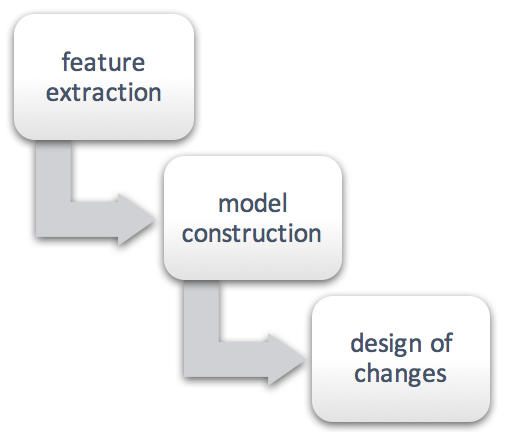
\includegraphics[scale=0.6]{images/02-art/oppmodelproc.png}
  \caption{Basic work-flow for designing systems able to implement any kind of modeling of co-existing agents for competitive advantage.}
   \label{behaviorModWorkFlow}
\end{figure}

It is not a secret that in order to be able to increase the likelihood of winning a game one should also consider the extraction of knowledge from opponents in the environment. Opponent modeling \textit{per se} is seen as the attempt to predict and identify behaviors of co-existing adversarial agents and propose appropriate countermeasure actions toward maximizing a given utility~\cite{fathzadeh_opponent_2007}.

In the Robot World Cup Initiative (RoboCup) a body of research has been done in the last decade trying to address the problem of opponent modeling. The RoboCup is a multidisciplinary initiative for building a team of robots capable of playing soccer. In this scenario, opponent modeling concepts are seen as an important requirement for building a competitive team and also as a growing research topic not only on this domain but also in the general multi-agent system area~\cite{rofer_overview_2012}. 

Since in most cases game history data is available, in either categories, researchers have extensively used data mining and machine learning techniques in order to construct off-line model of opponents which could them be used as classes in a kind of ``prediction phase'' during actual game play. Often, this prediction phase basically means: try to match the current observed opponent behavior to one the existing models for then try to adjust the internal behavior parameters accordingly. This matches the basic work-flow scheme in figure~\ref{behaviorModWorkFlow}.

Some important contribution to the problem has been done by~\cite{fix_behavior_2000,riley_recognizing_2002,riley_coaching_2001,riley_planning_2002}. In~\cite{riley_recognizing_2002}, the authors explored the domain of RoboCup by studying how to improve their agent team by constructing a probabilistic model representing predicted opponents' locations given the recent history of ball's movement and initial team members' locations. As common in this scenario, their approach focused in the use of a ``coach'' agent, enabled with a number of predefined models and a centralized view of the world, whose main role is that of communicating a plan to the rest of the team. The big idea is to taking into consideration the models' match with the observed data in order to predict opponent general behavior. 

The main assumption made by the author was that of opponent behavior being generated from a sample drawn from the predefined models given to the coach. Naturally, given the predefined models, it is still a challenge to decide which model best describes the opponent at run-time. As in the common supervised learning paradigm, they assumed the opponents will behave similarly to how they performed in the past, and use that information to develop a plan. In all of the models used, the distribution of each players final position was represented by a 2-dimensional Gaussian with equal variance in all directions. On successive works~\cite{riley_coaching_2001,riley_planning_2002} the authors managed to improve the online model selection through a kind of Naive Bayes approach focusing on plan representation and execution expressing spatial-temporal relations. 

An interesting observation made by the authors, also pointed out in~\cite{rofer_overview_2012}, is that during the plan execution it was not possible to take advantage from single unpredictable opportunities that may emerge. For instance, the agents would follow the plan strictly even if there is a clear chance of being successful against the opponent team by taking an immediate off-plan action. It is important to observe how this issue may direct affect the efficiency of autonomous agent involved in a PIRG. I understand that it is extremely necessary for the agent to keep a closer loop with the environment, paying attention to every observation that may emerge as opposed to always blindly follow a prescribed solution. Naturally, this pave the road for solutions that are able to represent some degree of belief regarding plan execution and revision. A possible solution to this issue was also pointed out by the authors. They basically suggested to store alternative plans and intelligently add monitors for these plans as in~\cite{veloso_rationale-based_1998} so that they could make the plan execution opportunistic~\cite{riley_coaching_2001,riley_planning_2002,rofer_overview_2012}.

In ~\cite{iglesias_comparing_2006} the goal was to use of statistical dependency tests for the identification of significant sequences from which to relate states to chains of events. Their underlying assumption was that observed team behavior can be transformed into a sequence of ordered atomic behaviors. In the follow-up work~\cite{burgard_classifying_2008}, sub-sequences inside sequences of behaviors are analyzed by using a frequency-based method. The big aspect presented on their work is that the model of an agent behavior is represented by a distribution of relevant sub-sequences. The behavior classification procedure is done using a modified Chi-square Test. Further improvements descibed in~\cite{iglesias_winning_2009}.

\cite{steffens_feature-based_2003, steffens_similarity-based_2005} studied the application of feature-based models for representing opponent behavior. In~\cite{steffens_feature-based_2003}, the gist of his approach comprises the identification of few features that could be observed by raw sensor data during game play, which diverged from~\cite{fix_behavior_2000} whose method stored every observation on the models. Those features were classified by using a Bayesian method, then a knowledge base is used in order to respond to what has been classified, i.e, select the appropriate strategy. One example of such features were the use of text-based description for in-game situations, like: ``The opponent often does long passes along the left wing to the forwards''. The methodology investigated in the paper turned out to be further studied to the extent of the use of Case-based Reasoning in~\cite{steffens_similarity-based_2005}. In this follow-up research, Steffens was able to identify some gain in classification accuracy showing that similarity-based opponent modeling can benefit from domain knowledge~\cite{rofer_overview_2012}. Case-base Reasoning, however, is likely to lead to high computational costs given the large number of cases do be retained in a highly dynamic environment~\cite{ahmadi_using_2004,rofer_overview_2012}.

In \cite{kaminka_learning_2003} their technique translates observations into a time-series of recognized atomic behaviors. For instance, given a stream of raw observation about the team members' position and orientation plus the position of the ball, their approach would recognize soccer-playing behaviors (passes, dribbles, etc..). Unlike other efforts, they did not care about how the low-level behaviors combine together for generating high-level strategies.  

\cite{ledezma_predicting_2002} also formulates the problem of opponent modeling as a classification task. In tacking the problem they proposed the decomposition of the learning task into procedures: the learning of the action name (passing the ball, kicking), and learning the parameters of that action. A follow-up work~\cite{ledezma_predicting_2005} studied the subject further by implementing machine learning to create modules that is able to infer the opponent's actions by means of observation. Their method, was called ``Opponent Modeling Based on Observation'' (OMBO) and was designed for two make improvements in two pathways: First, tacking the creation of a generic module (Action Labeling Module) that is able to label the last action (and its parameters) performed by any robosoccer opponent. This happens via the observation of another agent .The justification for this method is that agents generally do not have access to input/output pairs of events generated by a given agent. So, the approach must rely on sensor inputs only. Second, there is the construction of a model of the other agent based on the acquired data from the first module. This is what they called ``Model Builder Module''. In ~\cite{ledezma_ombo:_2009} they further discussed the applicability of the OMBO method giving a proof-of-concept of when learning a model of two different goalies. The idea was that their team striker gets as close to the goal as possible, and shoots when the goalie is predicted to move, i.e, by anticipation of the opponent movement. Figure~\ref{OMBO_model_task} presents the holistic view of the method found on ~\cite{ledezma_predicting_2005,ledezma_ombo:_2009}. The reader is invited to see how it relates do figure~\ref{behaviorModWorkFlow}.

% \begin{figure}[htp]
%   \centering  
%   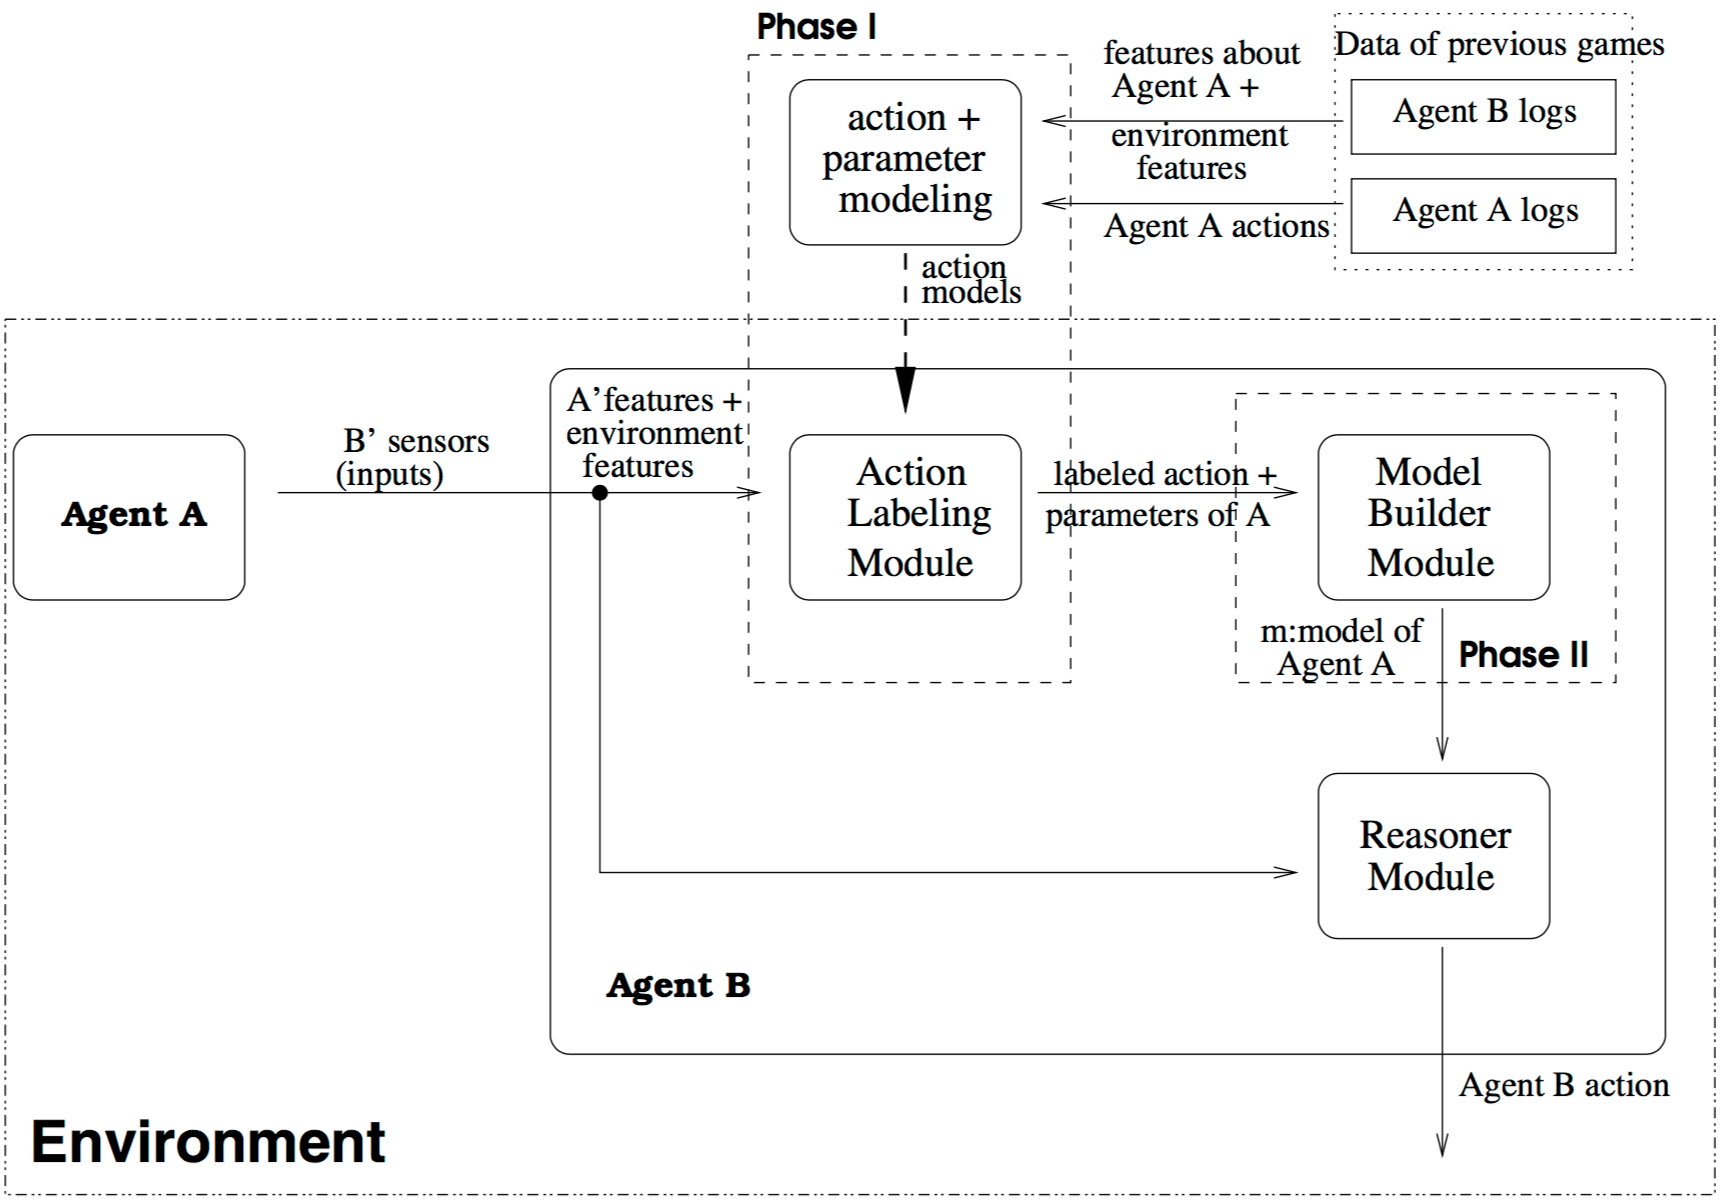
\includegraphics[width=\textwidth]{figures/OMBO_model_task.png}
%   \caption{The approach carrying out the modeling task in two phases: Action Labeling and Model Builder; in~\citet{ledezma_predicting_2005,ledezma_ombo:_2009}}
%    \label{OMBO_model_task}
% \end{figure}

Using data mining in order to define models of opponents in an off-line manner is the ideal scenario of an agent learning a model of other agents' behavior via direct observation of their past actions. However, that is only somewhat reliable when agents have many repeated interactions with one another or when the assumption of similar behavior between agents holds, otherwise it is somewhat hard to obtain any good generalization~\cite{stone_defining_2000}. Given the characteristics of the domain (physical interaction between agents), one may realize that the notion of proximity is quite important\footnote{proximity is a notion that basically relates to how close/distant interacting entities. It this turns out to be an ubiquitous notion even in simulated physical interaction as that showed in games.}. Often, authors try to somehow exploit proximity aspects as well as the spatial-temporal relations with certain property of the environment, for instance, the domain an agent exert over a field region (e.g,~\cite{riley_empirical_2002}). Obviously, proximity is not enough, but when combined with other aspects, like timing aspects, it is possible to get good estimates about the behavior of agents in their attitude with respect to in-game tasks. This trend is going to be present on the majority of papers focusing behavioral modeling.

When tackling team formation, one may observe that a large number of machine learning techniques has been tested in order to improve countermeasure actions for a specific team. Again, most of the methodologies used log files for the purpose of off-line learning of important characteristics. Neural Networks, for instance, has been extensively used for identifying the position of opponent team members with respect to given preset formations. After identifying a given formation, a plan could be transmitted by the coach agent to the rest of the team all for the purpose of performing the appropriated counteraction~\cite{nakashima_off-line_2010,ramos_discovering_2008, faria_machine_2010, visser_recognizing_2001}.

%Much work has centered on the problem of role allocation. That is to say the task of correctly allocating players to in-game roles that are appropriate for their capabilities also by smoothly exchanging team members between formation roles.~\citet{sukthankar2007policy} is an example of such effort. In their work ~\cite{sukthankar2006simultaneous, stone_task_1999}

For a in-depth overview of opponent modeling in RoboCup the reader is invited to refer to~\cite{rofer_overview_2012}. In the work the authors classify methodologies into two categories which basically comprise \begin{inparaenum}[\itshape a\upshape)]\item``formation modeling'', as it stands for the task of modeling team plays under the umbrella of collective behavior, and \item``individual behavior modeling'', which is related to the idea of modeling a single opponent agent\end{inparaenum}.

\subsection{Commercial interactive environment}

Virtual games have enabled a large amount of research effort into the design of player modeling methodologies. This is due to the increasing need for making Non-player Characters (NPCs) believable, i.e, make them resemble human behavior by implementing similar (to human) deductive reasoning process for action selection.  In summary, the need of such ability in virtual games is at least due to a few main facts: \begin{inparaenum}[\itshape a\upshape)]\item the growth as a commercial product; \item the increasing complexity; as well as \item the need for developing games that can exhibit a major level of intelligence and adaptive behavior (personalization)\end{inparaenum}~\cite{bakkes_personalised_2012}. 

An increase collection of papers has been published trying to address the problem of predicting the player (opponent) behavior (actions) in different levels and in different contexts. Focusing on opponent modeling, ~\cite{herik_opponent_2005} presented an overview of efforts for commercial games. In this work, they emphasize types and roles of opponent models, such as ``speculation'', ``tutoring and training'' as well as ``mimicking characters''. In ``speculation'', the idea is that some kind of heuristic (or utility function) -- such as minimax in zero-sum games like chess or checkers -- is used in order to assess the quality of available opponent's actions during game-play. In simple terms, this relates to the idea of using knowledge of the opponent's preferences or skills in order to drive the game into positions/states that are considered to be \textit{less favorable} to the opponent. This is the same core idea behind the approach described in~\cite{markovitch_learning_2005}, where they defined the concept of \textit{opponent weakness} (as a quantifying measure) together with a method for learning a model of this concept. The key-point in~\cite{markovitch_learning_2005} was the care about the potential harm of modeling error and the incorporation of their concept as an extra feature in the decision process, not as the core itself.

Another example of such modeling type is the research done by~\cite{missura_online_2008} where the authors proposed to rank available actions for the player (at each turn of the connect four game) as to find a way to balance the behavior of the computer-controlled agent to that of the human player. The aim was to estimate the player's expertise, when looking at the history of moves performed, and by assessing their quality (rank) based on a minimax approach.  Thus, at each turn, they could make their agent select only actions that have similar rank to that of the player\footnote{Despite the fact~\cite{missura_online_2008} is mentioned here as an ``speculation'' type of opponent modeling -- since there's a kind of simulation procedure for evaluating the player's quality of movement -- one may also see the work as an effort for tailoring the game for optimizing gaming experience, i.e., a kind of difficult adjustment approach (cf. section~\ref{DDA}).}.

Tutoring and Training is seen in~\cite{herik_opponent_2005} as a type of opponent modeling that has to do with the assistance of a human player. For instance,  a model of the human opponent may be construct as to teach him how to achieve certain in-game goals in a personalized manner. This is ideal for \textit{serious game} environments where the player is confronted with a simulation of real-world events while trying to solving a potential real-world problem. Even by knowing that serious games can be entertaining, in this scenario the main purpose is essentially to train or educate users, thus, coming up with models that helps the game steer behavior towards those aspects are definitely important. In this context,~\cite{ha_goal_2011} tried to identify player's goals in the game Crystal Island -- a non-linear educational game about microbiology -- by using Markov Logic Networks\footnote{a probabilistic technique comprising a set of weighted first-order logic \textit{formulae} that enables uncertain inference over ``traditional'' binary logic. }. Goal recognition is assumed to be an important piece for player modeling and generally tries to identify the user's goals from a set of low-level observation (abduction)\footnote{Also related to goal recognition are techniques like plan and activity recognition, both well-known problems in general AI~\cite{ha_goal_2011}.}. 

The study in~\cite{ha_goal_2011} follows previous work on goal recognition (such as~\cite{mott_probabilistic_2006}), but under a much broader view: that of having individual goals not independent from one another (which turns goal recognition into a classification problem) and that of having ambiguous causality effect between actions and goals. In terms of features for player actions, they targeted three properties: \textit{action type} (e.g, moving to a place), \textit{location} (game place where the action was taken), \textit{narrative state} (player's progress in the game narrative).  Once again, model parameters are learned from corpus of data collected from the environment. Their results were compared with two baselines based on \textit{unigram} (a model that predicts goal based on the current player action) and \textit{bigram} models (makes prediction based on previous action as well) obtaining a 82\% improvement over them.

In~\cite{herik_opponent_2005}, the ``mimicking characters'' type is said to correspond to the observation that the virtual game is designed to be, above all, fun and entertaining, as opposed to play as strong as possible all the time. This amounts to the well-known observation that when performing a companion role, for example, the agent must do what is possible to behave in accordance to the expectation of the player, otherwise the human may lose interest in the game. Thus, this requires a model of the human in order to be effective. Also, in a PIRG scenario, this is an important aspect that would enable advancements in the interaction as a whole since the behavior of an autonomous agent should be dynamic enough to adjust to the individual experience. The central point is that of not designing static behaviors that are likely to be exhaustively exploited by the player. This type hugely overlap with the ideas of player modeling for creating a balanced game play, i.e., adjusting the game for the player individual experience. This subject is brought back on section~\ref{DDA}.  

Often, games and simulations provide access to full-observability of in-game events and player's actions. When this is somehow not true, there may be a (often large) corpus of data from usage history that is available for information extraction. This, naturally favors the use of off-the-shelf data-mining algorithms that are able to be put together easily and tested multiple times. However, on the design of PIRG, specially on a brand-new project, one may suffer from the lack of data for constructing off-line models of players. To get around this problem there exist at least two main alternatives: \begin{inparaenum}[\itshape a\upshape)]\item setup a data collection procedure, for example, by designing a first version of the game, implementing it and then collecting data in order to refine the game design; or \item invest on online procedures that are able to extract features from the player and come up with models of player behavior on run-time\end{inparaenum}, this later, of course, is undoubtedly much harder to face.

In PIRG, it may be possible to design methods that account for the evaluation of the current state in order to know which are the corresponding chances of winning/losing at the moment allowing for planning ahead ways to overcome/support in case of need. However, it is worth to salient the general constraints perceived in the domain, such as those from computing complexity, mobility, perception. As part of the domain definition it has been suggested the necessity for designing PIRGs via the use of low cost platforms which commonly have limitations regarding computing power, energy consumption and others. Indeed those constraints must be taken into account if there is the clear goal of making PIRGS reach the market~\cite{martinoia_physically_2013}.

Competitive advantage and/or experience optimization (section~\ref{expOptimization}) are not the unique types of approaches. There were also attempts for classifying opponent behavior to the extent of helping in the design of the game itself. An example of this is the work of~\cite{etheredge_generic_2013} where it is possible to see the implementation of fuzzy cluster analysis and Hidden Markov Models (HMM) for finding player styles. The approach works as  player behavior\footnote{defined as a sequence of game actions.} classification method that consists of three components: Interaction Registry, cluster analysis and HMM. The first, serves as a data storage for actions maintaining a cumulative score value for them. The idea behind this is that actions that are not frequent are going to have an exponentially decreasing value in importance. On the other hand, frequent used actions have high importance score. Those importance values for actions then constitute a primary source of information that is going to be used by the cluster analysis as a way to group, i.e. classify, player's style. HMM is subsequent used during game-play aiming to classify new players, as they play, and helping to spot appropriate and dependent game adjustments. The author claimed their method would be able to be used across different games (given their definition of player behavior) which can help as a possible generic design-tool.

Using the Rush 2008 American football simulator~\cite{laviersa_using_2014} introduced methods for performing predictions about the players' physical movements when learning team policies. When focusing on recognition of team play they investigated the use of support vector machines, an optimal margin classifier commonly used in supervised learning problems. They trained SVMs for a multi-class objective by using a collection of simulated games under controlled conditions, so they got instances of every possible combination of offense and defense plays from a number of team starting formation configurations. The output of the play recognizer was defined as the system's best guess (at the current time step) about the opponent's choice of defensive play. Thus, they could use this information to select the most appropriate offense.

Also in~\cite{laviersa_using_2014}, the authors focused on proposing methods for discovering how to effectively  subgroup agents together so to accomplish a given formation task, similar to~\cite{stone_task_1999}. Here again they based their method on an analysis of game data from successful team plays. The idea was to implement a supervised learning mechanism in order to identify important group of players w.r.t. each play. It is interesting to mention the three general types of cues that were used for the purpose of subgroup extraction: \textit{spatial} -- i.e, the constant relationships between team members over a period of time; \textit{temporal} -- co-occurrence of related actions; \textit{coordination} -- dependencies between members' actions. Those cues turn out to be basics features from most types of approaches in the discussed scenario. Undoubtedly, a larger number of papers has been focusing on player modeling for improving playing experience as to maximize the chances of maintaining the player engaged. This is the topic of discussion of the next section.

%In~\citet{vanderheijdendynamic} they discuss an approach to organising units in a Real-Time Strategy games. They start by learning the effectiveness of a formation in actual play and then directly applying learned formations according to the classification of the opponent player. The feature-space describing formation were, among others, spatial characteristics between unit members (such as horizontal and vertical distance), speed, number of possible formations (among predefined one), combat behavior (rules for employing the behavior). When classif

\section{Modeling for experience optimization}\label{expOptimization}
In virtual games player modeling is best defined as the study of the use of artificial and computational intelligence techniques for the construction of models of players in dimensions regarding behavior, cognition and affective state as well as beyond-game high level aspects spanning personality and cultural background~\cite{yannakakis_player_2013}. The idea behind such models is related to the goal of enabling a game to adjust the capability of its components and attributes towards an individual player satisfaction~\cite{herik_opponent_2005}. This idea has largely increased in importance over the last years. As one of the central reasons for that is the increasing complexity of modern games fostered by the enhancement in computing power and graphics, as well as the commercial strategy of personalizing gaming experience~\cite{teng_customization_2010, herik_opponent_2005}. This section discusses the dimensions mentioned in the definition, namely: \textit{cognition}, \textit{behavior} and \textit{affection}, describing their main characteristics and supporting work.

\subsection{Focus on cognition and theoretical models of behavior}
One way researchers have addressed player modeling in games is by relying on theoretical frameworks mainly supported by psychology and neuroscience factors~\cite{yannakakis_player_2013}. By doing so, cognition aspects -- broadly seen as a set of all mental abilities and processes related to knowledge, such as: attention, memory, evaluation, reasoning, problem solving and decision making, learning and so forth~\cite{wiki:cognition} -- are often investigated. 

Researches focused on theoretical framework of behavior are described in~\cite{yannakakis_player_2013} as being model-based. In this sense, they follow the \textit{modus operandi} of humanities and social sciences which work, according to the authors, by coming up with a hypothetical model in advance that is investigated in relation to what extend it fits the observations. When concerning the development of engaging experiences in entertainment systems,~\cite{yannakakis_how_2008} states that a comprehensive review of the literature regarding the elicitation of qualitative features and criteria derived from experimental psychological studies reveal a tendency of overlapping with the exploitation of theories of \textit{fun}, such as those discussed in~\cite{malone_what_1980, lazzaro_why_2004, koster_theory_2013} envisioning to drive game design, as well as \textit{flow}~\cite{csikszentmihalyi_flow:_1991} -- which is traditionally used as a way of evaluating player enjoyment~\cite{sweetser_gameflow:_2005, cowley_toward_2008} (Fig.~\ref{flowDiagram}) -- and concepts like \textit{immersion}~\cite{calleja_digital_2007}. Most acceptably, according to theses theories and concepts, player engagement is most related to factors such as challenge, curiosity and fantasy.

\begin{figure}[htp]
  \centering  
  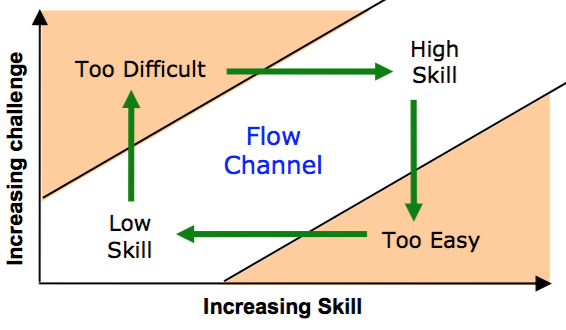
\includegraphics[]{images/02-art/flowDiagram.png}
  \caption{A flow diagram from~\cite{hunicke_ai_2004}. The figure shows the relationship between skill and level of challenge derived from the theory of flow~\cite{csikszentmihalyi_flow:_1991}. The point is to keep those two dimensions in a kind of positive correlation, meaning an increase that roughly approximates the diagonal.}
   \label{flowDiagram}
\end{figure}

Models aligned with cognition theories are seen as a valuable opportunity for understanding what the user is thinking when playing, which has direct relation with the ultimate desire of making the game respond intelligently to the player. Supported by~\cite{bohil_cognitive_2007}, the fundamental advantage of a direct focus on modeling principles embodied in a theory of cognition is that it provides dynamic view at the individual player level, since it is possible to make statements about attention, learning, decision strategies, biases, an so on, unraveling indicators of the mental underpinning of observable behavior. 

The design of better NPC's, for instance, is one of the central areas positively affected by the focus on cognition~\cite{funge_ai_1999}. Intuitively, once it is possible to measure some cognitive-related characteristics in the player (e.g., the attention level with respect to some in game resource) it is possible to use them to steer the NPC behavior towards the improvement of a desired AI capability -- Adaptive difficulty adjustment is one of those capabilities. Indeed game difficulty is seen as having a direct link between challenge and fun, acting as source of satisfaction~\cite{koster_theory_2013,yannakakis_modeling_2006} (cf. section~\ref{DDA}). 

Cognitive models of players were also investigated with respect to psychological and cognitive neuroscience motivated question trough assessing physiological and/or psycho-physiological states during play. For instance, brain imaging techniques have been used to understand brain activity patterns related to aggressive thought stimulated via violent game content in~\cite{weber_does_2006}. The work of ~\cite{baumgartner_neural_2006} used Electroencephalography (EEG) combined with psychometric measures, as a first attempt to investigate neurophysiological underpinnings of spatial presence\footnote{spatial presence is considered as a sense of being physically situated within a spatial environment portrayed by a medium, such as television and virtual reality.} triggered in different virtual roller coaster scenarios.

Optimistically, as seen in~\cite{bohil_cognitive_2007}, the major point in cognition or related framework-based approaches for player modeling is to discover which model inputs\footnote{in the sense of a parametric representation of cognition aspects.} place, for instance, unrealistic demands on a specific cognitive function, such as attention. Successful results on this, might heavily equip researches and game developers with valuable guidance for narrowing the range of necessary resource-consumption when aiming for desired results.   

\subsection{Focus on in-game actions}
A classical trend in player modeling is that of understand how primitive in-game activities are responsible for comprising the player's general behavior. Originally, the first attempts for modeling players in this context used classical zero-sum board games (like chess, checker and go) as test-beds mainly by implementing search/heuristic methods for find best moves in the game-tree. According to~\cite{bakkes_player_2012}, since tree-search techniques use evaluation functions in order to assess the pay-off of a particular move, they may be consider player models.

In-game actions are building blocks for any standard behavioral modeling approach. Most commonly, primitive (or low-level) actions are the unique way available through which it is possible to identify player's preferences and decision-making style as well. Additionally, this modeling dimension is transferable across different game genres. A sequence of low-level actions -- such as moving to one direction to another -- is generally related with a classifiable behavior, such as ``attacking'', ``defending'', ``fleeing'', etc. In the RoboCup soccer league, for instance, a sequence of actions comprising targeted movements towards the opponent goalie may be commonly (and generally) classified as an ``attack''. Similarly, a sequence of actions intending to systematically prevent the opponent team from advancing on the field may be characterize as a ``defensive'' behavior. From this example, it is quite natural to realize that actions encode behaviors by perhaps acting as a kind of representation language for them. The important bit is that by keeping track of actions performed it is possible to find patterns that can be reasonably grouped together under the concept of a specific behavior\footnote{as discussed, actions were the raw information in most modeling approach for competitive advantage in section~\ref{compadvantage}.}.

Although classifying behaviors in this way may be relatively easy for simple full-observable environments, involving a few possible deterministic actions and abstract behaviors, this classification process is limited in modern complex games since they normally have a large state-action space. Also, behaviors commonly lack the existence of a clear crossing point between them what makes it challenging for the construction of player models. Giving the size of the state-space, researchers have also to deal with the uncertainty involved in the fact that different action sequence may converge to a same behavior while having a close relation with others. The notion that action sequences may be noise, is important at the same proportion that it is also a challenge that has to be taken into account when using low-level actions for modeling behavior.  Furthermore, while computational constraints (such as memory demand) are the big key points for some case, for instance, in search methods applied to turn based games, the dynamic characteristics in other types of games is the key instead. In PIRGs, the inherently dynamism of the environment demands a special treatment on those aspects.

Besides all computational constraints involved and discussed on the previous paragraph, one might also see fit the necessity of having different levels for behaviors. For instance, one might be interested on identifying when the player is attacking mindless or when the player is using a full-fledged plan for performing the attack. In this context, what is the boundary characteristic that separates those two behaviors? Again, using the RoboCup soccer league as an example,~\textit{is the player engaged in a proper ``attack'' or just keeping the ball in the attack field perhaps for the purpose of spending time?}\footnote{Note that a ``proper'' attack may have more structured actions, perhaps comprising well-know patterns as opposed to a behavior of just ``spending time'', which in this case may use different sequence of actions.}.

The work of~\cite{bakkes_player_2012} presents an extensive discussion about the use of actions for player modeling envisioning game experience optimization. In the author's understanding, actions models seem to be an attractive possibility of a model since once being able to predict accurately the future actions to be taken by the player, acting accordingly would be a relatively easy task. However, they agree that the use of such models are limited unless when applied to relatively uncomplicated games. The justification for that is also related to the complexity of state-action space in state-of-art games. The authors, also deem three more subdivision of for the topic, described on Table~\ref{actionModels}.

\begin{table}[!ht]
\centering
\caption{The proposed classification by~\cite{bakkes_player_2012} for dimensions used in player modeling techniques based on virtual in-game actions.}
\label{actionModels}
\begin{tabularx}{\textwidth}{|c|X|} \hline
\textbf{Type of model}&\textbf{Brief description}\\ \hline
Tactic-based & relates to the automatic identification of short-term behavior as composed from actions targeting the achievement of a specific local goal. A common well-exploited concept is \textit{formation of game characters} which can be defined as a disposition of certain game agents.\\ \hline
Strategic-based & concerns global-term game behavior assessed via tactics sequences. This behavior may span over the entire game, some iterations of it or even across distinct genres of games.\\ \hline
Profiling-based & concerns psychological motivation for tactics and strategies.\\ \hline
\end{tabularx}
\end{table}

The divisions presented in Table~\ref{actionModels} are, in fact, not mutually exclusive and one can see them in a loose hierarchical manner. In other words, tactical-based models depend on action-based ones and, in the same way, strategy-based models may comprise a behavior inferred with the help of the previous two, etc. The main advantage, of modeling tactics over actions, however, is that the state-space complexity decreases as a result of higher information abstraction. But, since they are interrelated with each other aiming to achieve an overarching goal, modeling tactics alone, according to the authors, is not enough for effective modeling player behavior since strategic play assumptions, as a high-level motivation for tactics, is commonly not incorporated, therefore, those models cannot generalize well over the underlying intentions behind observed tactics.

Additional to the use of actions in the modeling context discussed in section~\ref{compadvantage}, they are also the raw material exploited on designing games that can adjust difficulty automatically in order to keep the player's engagement at a high. Specifically, along-side procedural content generation -- the concept of generating game content on the fly -- automatic difficult adjustment (DDA) has taken a large piece of the virtual game community.

In essence, the idea is pretty simple: start by measuring the player's skill or level of challenge (difficulty) at a given moment and based on that steer the game behavior towards a state much likely to be compatible (in skills or challenge level) with that of the player. Following this recipe, Andrade et al.~\cite{andrade_online_2004, andrade_extending_2005} aimed at investigating the usage of Q-learning and a challenge function in a 2D fighting game scenario. In their work the authors came up with a challenge function strictly based on the difference between the NPC and player's health. From this, a game is assumed to be balanced if the function fluctuates around zero. By using a regular Q-learning they get to choose different best actions so to force the algorithm to choose the ones that most likely, according to the challenge function, matches the perceived player skill. 

~\cite{hunicke_ai_2004}, in turn, addressed DDA by considering the notion of inventory analysis, that is, the processes of analyzing what resource are immediate available to the player w.r.t. the current challenge level of the game. During the game process, they observe certain player's characteristics, for example the level of damage the player takes, in order to generate an indicative for the necessity of system intervention. When needed, their system would adjust supply and demand or resources so to control overall game difficulty. Ideally, the authors target the reduction of necessary intervention so to make those as seamless as possible. The system aims at keeping the player at the flow channel~\cite{csikszentmihalyi_flow:_1991} by encouraging certain events to take place or not. For example, the system basically tries to predict when the player is repeatedly putting himself on a state whee current means can no longer global or local goals. When this happens, the system intervene helping the player progress.

Not surprising, the notion of having a ``challenger function'' that helps to guide adaptation is pretty much ubiquitous in the adapting game literature. Furthermore, any system relying on DDA should also be concerned about the timing implication of such technique, i.e., the implications regarding the good moment to perform an attempt towards adjusting the game. For beginners, this is because a high frequency of adaptation is more likely to give the appearance of instability and so cause the game to be perceived as random. This instability is often referred to as the ``rubber-band'' effect as the IA appears to wobble around its skill level if the (human) player is too good and, conversely, overrun the player when he plays equivalent to the AI. Here though, appears clear the difficulty involving designing challenger functions. In the experiments done by~\cite{hunicke_ai_2004}, the authors noticed that an reactive approach, i.e. adjustment of onset elements, may run the risk of disrupting the player's sense of disbelief contributing to make the interpretation of the game harder and also make it ``schizophrenic''.

In Hagelbäck et al.~\cite{hagelback_measuring_2009}, the authors went further on pooling people's opinion for the sake of knowing if playing an even game is more entertaining over being superior all the time. On their case study 60 people participated and they took the opportunity to conducted experiments using static and dynamic agents for their game test-bed. The dynamic agent type was able to react to in-game player behavior (for instance, to the player losing game units). The results gotten from their research suggested the dynamic agents were most entertainment to play, at the same time the static ones presented themselves as too easy or too difficult. From here, I see once more the supporting evidence for justifying any effort in constructing efficient DDA-based systems for the purpose of keeping interactions. Despite the fact there are intuitive justifications, experimental results cover a fraction of the driving force behind such effort.

\cite{spronck_-line_2004} is one of the most popular example of player modeling in virtual games. In their method, called ``dynamic scripting'' and defined as an unsupervised online learning technique for games, they maintain several rulebases, one for each class of computer-controlled agents. Rules in the bases are manually designed using domain-specific knowledge and every time a new agent of a particular class is generated, the rules that comprise the agent script are extracted from the corresponding rule-base. In this approach, the probability that a rule is selected for a script is proportional to the weight value that is associated with the rule. Also, the rulebase adapts by changing the weight values to reflect the success or failure rate of the associated rules in scripts.

It did not take long until researchers realize using a challenge function would be able to pave the way for black-box optimization algorithm. Much of the time the literature covers the attempt on using evolutionary techniques as the main technique for DDA. Among those work, it is worth noticing~\cite{olesen_real-time_2008} from which the authors use evolutionary techniques to evolve agents so to balance an estimated challenge rating for the player skill. The take-away idea is that of making agents with a minimal difference in skill (w.r.t the player) to survive more and, on the other hand, lower the fitness of the ones whose difference is larger.

~\cite{demasi_-line_2003} focused on the use of co-evolutionary algorithms (CEAs) proposing some methods and strategies for online evolution in an action (real-time) game. In this game, the NPC is evolved towards improving difficulty levels of gameplay. The author present four different methods: one that uses game specific information; one that merges offline-evolved data with online evolution; an two others that focus on using online data only and using offline and online data together. Considerable drawbacks in the approach are the slow rate of learning and the one-direct way of evolution, always toward the optimizing behavior.

\cite{sejrsgaard-jacobsen_dynamic_2011} took a different approach by using Behavior Trees (BT), a kind of hierarchical finite state machine for controlling NPCs, in order to dynamically adjust the difficulty in a 2D fighting game. They basically tested two different approaches. First, the traditional approach of defining predefined behaviors (encoded on BTs) and finding a way to switch between models (behavior) at run-time. For this, they developed an algorithm for selecting BTs based on perceived conditions. The second method, however, adjusts difficulty by changing BT properties themselves at run-time, such as the probability associated with children of selector nodes. This last method, was the one that obtained high capability in balancing the game. As claimed by the authors, their method served as a proof of concept for a small sized scenario (simple 2D fighting game) leaving the possibility for further investigation in larger game scenarios. Here, pops out an opportunity for testing on a PIRG context, perhaps by following the current trend on applying such technique in Robotics~\cite{scheper_behavior_2015, pereira_framework_2015, marzinotto_towards_2014}.

In summary, approaches addressing DDA must prior to the definition of the challenge function identify important game characteristics affecting game difficulty, i.e., challenge level. This is where the knowledge engineering resides. The overall philosophy is the adjustment of the game behavior to the perceived player's game skill, which should be done as seamless as possible. A good survey about adaptivity challenges in games and simulations is that of~\cite{lopes_adaptivity_2011}. The reader may refer to it in order to see a deeper treat on the identification and discussion of main challenges associated with the domain and also promising directions for research.

\subsection{Focus on affection aspects}\label{affectmodeling}
Also, some trend has emerged aiming on assessing the player's affective state (mainly emotion) as a mean of measuring the quality of interaction provided by the game. Here, the goal is related to the task of inferring internal traits of the player, such as personality and preference, during game-play~\cite{van_lankveld_psychologically_2009}. Methodologies that take this approach are more towards a research domain known as \textit{affective user modeling}, where the key point is that of assessing, heavily by using affection models, the inner state of the player regarding motivations for actions either based on action selection or through physiological data~\cite{van_lankveld_psychologically_2009}.

Being able to identify emotional profiles in this domain is useful given that they target a direct characterization of enjoyment level. For instance, after realizing that the player is compatible with an extroverted and highly responsible profile, the game AI may engage the user in rapidly and repeatedly shifts of events, like from calm situation to a long and intense chain of events, or even an steeper increase on motion abilities for NPC agents when proximity aspects, for instance, are important~\cite{bakkes_player_2012}.

Working on this,~\cite{tognetti_modeling_2010} proposed a framework to estimate player enjoyment preference from physiological signals in a car racing game. They collected 5 physiological signals from players using the propComp Infiniti device\footnote{\url{http://thoughttechnology.com/index.php/procomp-infiniti-308.html} accessed on March, 24, 2016.}, such as: Blood Volume Pulse (BVP) and Electrocardiogram (ECG), both sampled at 2048Hz, as well as Galvanic Skin Response (GSR), Respiration (RESP) and Temperature (TEMP), all of the three sampled at a rate of 256Hz. From those basic signals, they were able to extracted features such as: Heart rate (from ECG and BVP); magnitude and duration of GSR; expiration/inspiration time, apnea in/out time, respiration interval (all three from RESP); upper/lower envelope of BVP. Their data analysis, using Linear Discriminant Analysis (LDA), showed correlation between reported enjoyment and the described features, motivating further application on the use of biological signals without making any assumption on players' in-game activity.

Yannakakis and Hallam have published lots of papers on the matter of capturing and modeling affective state of entertainment, targeting children physiological state during physical game play. In~\cite{yannakakis_modeling_2006,yannakakis_entertainment_2008}, children's heart rate, blood volume pulse and skin conductance were analyzed in the Playware prototype playground~\cite{lund_playware_2005}. Their findings suggested that a higher average and maximum heart rate, a steeper blood volume appear to correlate with higher levels of reported entertainment in children of 8-10 years-old. Essencially, the main effort is related to modeling entertainment based on selecting a minimal subset of individual features that are able to construct the quantitative user model for predicting the children's reported entertainment preferences. In doing so, they tested Large Margin algorithms (based on the SVM principle) and Evolving Artificial Neural Networks. Successive works investigated feature selection and extend the approach for computer games~\cite{yannakakis_towards_2006,yannakakis_entertainment_2007,yannakakis_feature_2007,yannakakis_entertainment_2008B}. 

There are indeed plenty of papers proposing the use of physiological method in game research. A widespread understanding is that measures from those methods are known for providing sensitive ways to assess the game experience, but they are hard to deal with since very often they require controlled experiments. In order to know more about this trend of research, the reader may refer to~\cite{kivikangas_review_2011} whose work presents a review focused on psychophysiological methods for game research.   
 
\subsection{Existing review papers and taxonomies for player modeling in games}\label{reviews}
Taxonomies and reviews for player modeling has been also proposed recently. In~\cite{smith_inclusive_2011}, under the emphasis that ``player modeling'' is a lose concept\footnote{According to them, it can equally apply to everything from a predictive model of player actions resulting from machine learning to a designer's description of a player's expected reactions in response to some piece of game content.}, the authors introduced a broad taxonomy for the purpose of distinguishing between the major existing player modeling applications and techniques. Four facets were suggested: the scope of application, the purpose of use, the domain of modeled details, and the source of a model's derivation or motivation. The expectation involved is that the taxonomy would allow the identification of relevant player modeling methods for particular problems and clarify roles that a player model can take. As pointed out in the previous section, the work of~\cite{bakkes_player_2012} focus on player behavioral modeling via in-game measurement of the human player distinguishing four types of player models: actions models, tactical models, strategic models and player profiling. Through their examination, they noticed that those models are increasingly resource-intensive to construct, but they also have a increasing tendency to generalize better.

~\cite{machado_player_2011} also proposed and discussed a taxonomy for player modeling research gathering and organizing information from several different sources. They, in turn, tried to characterize the most important topics in the area expanding the discussion from~\cite{herik_opponent_2005} about the most common techniques, further presenting a new set of techniques. Additionally, they did an analysis of player modeling research possibilities in several game genres and also listed suitable game platforms for experimentation, discussing main characteristics.

Targeting a holistic view of player modeling with the aim of providing a high level taxonomy and discussion of key components of a player model,~\cite{yannakakis_player_2013} cluster the field into either \textit{model-based} approaches -- those that are built on a theoretical framework -- or \textit{model-free} ones -- those that refer to the construction of a model between player input and a player state representation by mainly relying on the modus operandi of exact science, through computational techniques related to AI and ML. Additionally, they present a discussion about inputs and outputs to computational methods described as well as applications and current key challenges the field faces which are correlated to the inputs and outputs to the mentioned computational models.

\begin{table}[!ht]
\centering
\caption{Summary of existing popular survey-like papers concerning player modeling. {\mycirc} stands for proposal of taxonomy, {\mystar} stands for overview of literature and {\mydtriangle}, in turn, correspond to survey or review.}
\label{summaryReviews}
\begin{tabularx}{\textwidth}{|c|c|X|} \hline
\textbf{Paper}&\textbf{Type}&\textbf{Brief description}\\ \hline
\cite{smith_inclusive_2011}	& {\mycirc} & Build a broadly applicable taxonomy that can describe player modeling techniques across all games , both digital and non-digital, and in all games genres.\\ \hline
\cite{bakkes_player_2012} 	& {\mycirc} & An overview of methods by detailing four distinct approaches for modeling behaviour of players, namely: modeling player actions, modeling player tactics, modeling player strategies and player profiling. \\ \hline
\cite{yannakakis_player_2013} & {\mycirc},{\mystar} & A holistic view of player modeling, a high level taxonomy and discussion of key components as well as a description of challenges currently faced in the topic.\\ \hline
\cite{bakkes_personalised_2012} & {\mystar} & Motivation concerns for the topic, an broader overview, and  adaptive components for personalised games\\ \hline
\cite{machado_player_2011} &{\mydtriangle},{\mycirc} & Presents a survey of the field, discussing the main concepts and proposing a general taxonomy. \\ \hline
\cite{karpinskyj_video_2014} & {\mydtriangle} & Highlight most relevant trends and directions of research for the task of designing personalisation in games.\\ \hline
\end{tabularx}
\end{table}

Focusing on the point of personalized game experience in general,~\cite{bakkes_personalised_2012} provides a motivation for the promotion of methodologies in the topic as well as an extensive overview of scientific literature. To the former objective, they describe psychological foundations, the effect of satisfaction, the advantages to game development and requirements for achieving ambitions. To the extent of the overview, they go pretty much in the same room of what has been exposed in~\cite{bakkes_player_2012}, however providing an intensive discussion about \textit{components of personalized games}, namely: space adaptation, mission/task adaptation, character adaptation, game mechanics adaptation, narrative adaptation, music/sound adaptation, player matching and difficulty scaling. An additional discussion about the relationship between personalized gaming and procedural content generation as well as the generalization to other domains (such as ambient games, human-computer interaction) is also mentioned.

Similarly, the work of~\cite{karpinskyj_video_2014} touches the subject of surveying the most relevant trends and directions of research in personalisation of computer games, in the extent that it is a true multi-disciplinary problem requiring contribution from areas as diverse as artificial and computational intelligence, game studies, psychology, game development and human computer interaction. Their survey correspond to five ways that, according them, players are often distinguishable from each other: by preference, personality, experience, performance and in-game behavior. Their discussion also aims to identify key research avenues that require further exploration.  

Table~\ref{summaryReviews} characterize the most important points in the mentioned papers. In summary, in this section I attempted to point out existing review that are useful to get more in-depth details about the discussed topic.

\section{A brief discussion on aspects of behavior and activity modeling for PIRG design}\label{DDA}

As discussed previously, a desired goal for PIRG design is to have autonomous robots able to adjust behavior towards optimizing the player experience. In the direction of achieving this result, one may see some sub-tasks that are fundamental to the problem, i.e., one must \begin{inparaenum}[\itshape a\upshape)]\item deal with the maximization of the player's expectation about the agent rationale -- allowing believable companion/adversarial roles to be effectively implemented; \item deal with timing requirements for the design of interaction -- since asynchronous actions may hugely impact engagement; \item feature selection; and \item modeling framework -- to the extent of selecting which one of the focuses presented on section~\ref{expOptimization}\end{inparaenum}.

\cite{bonarini_timing_2014} presented key aspects on timing issues he observed during the design of several robogames. Regarding those aspects related to the structure of the game:

\begin{itemize}
\item \textbf{Duration of the game}: This is a key-point since a game should reach its end in a time that guarantees to keep the players involved and to make them enjoy it. This greatly depends on the activity to be performed. In the PIRG case, the user's physical activity, i.e the workload, is the core of the interaction and given that it must be taken into account when defining the game duration so that the player can come to the end with a proper fatigue requirement. The reader is invited to think about the effect on engagement when this point is not well designed.

\item \textbf{Duration of an in-game task}: In a game, a set of tasks should be achieved. Naturally, the duration of such tasks has to be bounded by the duration of the game, or a game match. So, the duration of in-game tasks can be appropriately defined in order to provide some pressure on the players such that it may be likely to engage them, rise their interest, since an appropriate level of pressure and anxiety is related to challenge. The take-away idea here is that limiting the time available for an in-game task is a key-point to make it challenging.

\item \textbf{Duration of non-interactive activities}: In some games, there are activities that must be performed by a single player and so must have the right amount of time dedicated to them, i.e, a right period of time without any interaction from others (e.g, a solution of a problem, a recovering procedure). If those activities have to be done by human players, enough time has to be left for their accomplishment, but not too much time that could make them less challenging. On the other hand, if those activities must be performed by the robot(s), the human player should somehow be involved at the same time in some other activity, or the time dedicated to them should be short enough in order to lower the likelihood of making the human player bored, but long enough to be credible w.r.t. the storyboard of the game.
\end{itemize}

Some timing aspects related to the performance of both the human players and robot were also mentioned in~\cite{bonarini_timing_2014}.

\begin{itemize}
\item \textbf{Reaction time}: The time each player needs to react to an external event can be a constraint to be considered in game design. The human player's reactions in a physical interaction can be instinctive, thus requiring few hundreds of milliseconds to be activated, or may require some cognitive activity (e.g., reasoning, recognition), whose duration may span also some seconds. In PIRGs, since they are often designed for a lively interaction, the cognitive load is usually relatively small, and a time around one-two seconds for a cognitive response from the human player in a challenging situation is often considered as appropriate. The reaction time of the robot player mainly depends on the time to recognize a situation, which is related to the time required to elaborate signals, which in turn depends on the complexity of the data to be analyzed and on the available computational power. Since PIRGs are targeted in principle at a mass market comparable to the one of video games, the robots should be low cost, with simple sensors, and the available computational power might be as low as the one provided by cheap processing systems, like Arduino or Raspberry pi, up to that of an external laptop, tablet or smart phone. This might be a time constraint to be considered in game design, possibly justifying the related delays in the story.

\item \textbf{Actuation time}: Also actuation time may concern both the human and the robot player. For people, they might be constrained by some devices to dedicate time to perform an action (e.g., to perform a gesture with a WIIMote device). This might be desired to put some challenge in the game, and also to reduce the power of the human player w.r.t. that of the robot, so to make the game more even. For the robot, the actuation time might be a constraint given by the selected mechanical implementation, or might even be desired to reduce the power of the robot. For instance, if a robot could run fast enough to reach a target before a human player, it might be the case to reduce its speed so that the player can compete with it with some possibility to win.
\end{itemize}

Some other timing aspects are related to the establishment of a relationship.

\begin{itemize}
\item \textbf{Opponent behavior detection time}: Playing with artificial entities is engaging if the human player forgets the status of the opponent and attribute to it some human-like abilities. In particular, human players would like to play with entities that show some intelligence and intentionality. A way to achieve this status is to understand why the entity is performing an action, and, in general, what is its behavior, and what it aimed at. This may require an amount of cognitive activity proportional to the complexity of the behavior. In the mentioned experiments turned out that a random behavior is perceived as not interesting: the player believes that it is not worth to spend time with a silly entity. A too complex behavior is perceived as a random one, mostly because in PIRGs there is not much time to reason in a cool way on all the aspects of the perceived actions. The good behavior is one that requires a short time to be detected: not too short to consider the robot as ``too simple minded'' to play with, but also not too long to dismiss the cognitive activity of trying to understand it while the player is confronting the robot.

\item \textbf{Credibility}: Each action should have a motivation, and should be credible w.r.t. the perceived motivation. Timing of the action should be consistent with this. For instance, if the robot seems to take a decision about what to do, the consequent action should last until there is a good motivation to change it. For instance, if a autonomous robot would change its movement direction randomly, there would be no apparent reason to motivate the change, and the robot would be perceived as silly. This, of course, depends on the PIRG. In Jedi Trainer 3.0, for example, a random decision about the direction to take is consistent with what the robot is doing: trying to find a gap in the trainee guard.

\item \textbf{Activity pace}: Each player is assumed to do actions with a purpose for the game. Since they are interacting, the activity pace should be similar: a different pace, a different time between the selection of subsequent actions, would be perceived as if one would be favored w.r.t. the other one. Uneven games, in one sense or the other, are usually not appreciated.

\item \textbf{Timing perception}: In interaction, timing is a subjective perception, and it can be modified by the interaction mood, or media, or by external devices. If there is an exchange, its pace can be modified by a ``modeling and lead'' strategy. If there is a time limit to perform a task, the perception of its urgency might be increased again by taking a faster pace in all movement changes, or also by simply giving relevance to the time-to-end, e.g., by adding rhythmic lights, sounds, or clocks.
\end{itemize}

\section{Conclusions}

In this document, I have aimed on the presentation of relevant aspects and popular papers in the field of player modeling both to the extent of maximizing competitive advantage (section~\ref{compadvantage}) and experience optimization (section~\ref{expOptimization}). Despite the fact it is not supposed to be an exhaustive review of literature (for which the reader may refer to works pointed-out on section~\ref{reviews}), it was enough for enabling the spot of interesting aspects one must consider when trying to achieve similar goals on PIRGs. The motivation for this document was that of providing some insights -- based on related literature aspects -- for the design of adaptive behavior in PIRGs, which more broadly represents the student's effort on going through the literature in order to ease the selection of a first approach towards tackling this objective. 
